Do etapu przetwarzania wstępnego zaimplementowano algorytmy rozmycia i wykrywania krawędzi obrazu - przy pomocy filtru dolno- i górnoprzepustowego. Na etapie eksperymentalnym zaobserwowano jednak, że obrazy wejściowe w swojej domyślnej formie lepiej sprawdzają się w detekcji, przez co użycie filtrów stało się niekonieczne, przez co we właściwym procesie nie zostały wykorzystane. Efekty ich działań w celach poglądowych zaprezentowano jednak na Rys. \ref{fig:filtry}.

\begin{figure}[H]
\begin{subfigure}{.5\textwidth}
  \centering
  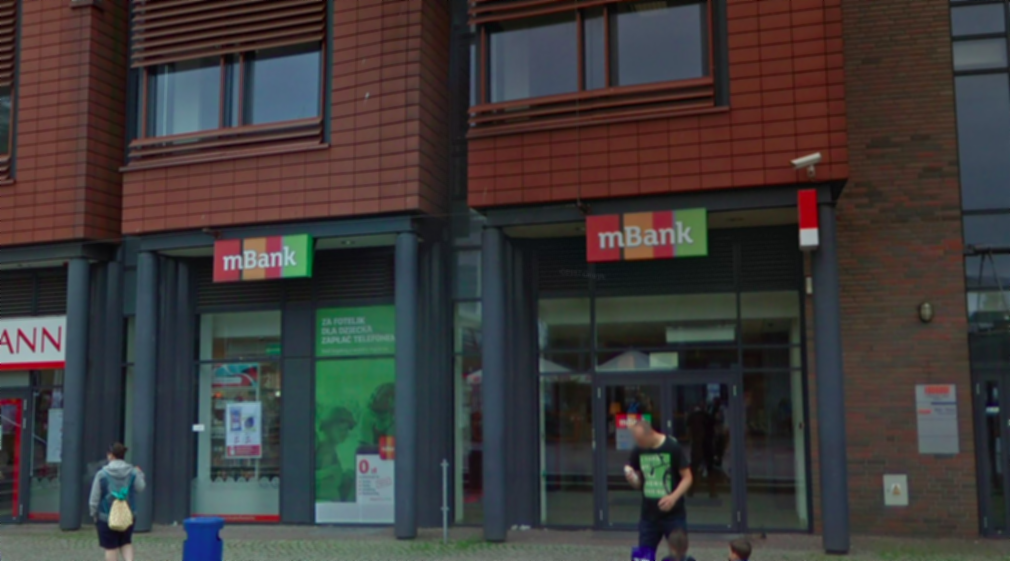
\includegraphics[width=.8\linewidth]{figures/img_blurred.png}
  \caption{Filtr dolnoprzepustowy - rozmycie}
  \label{fig:sfig1}
\end{subfigure}%
\begin{subfigure}{.5\textwidth}
  \centering
  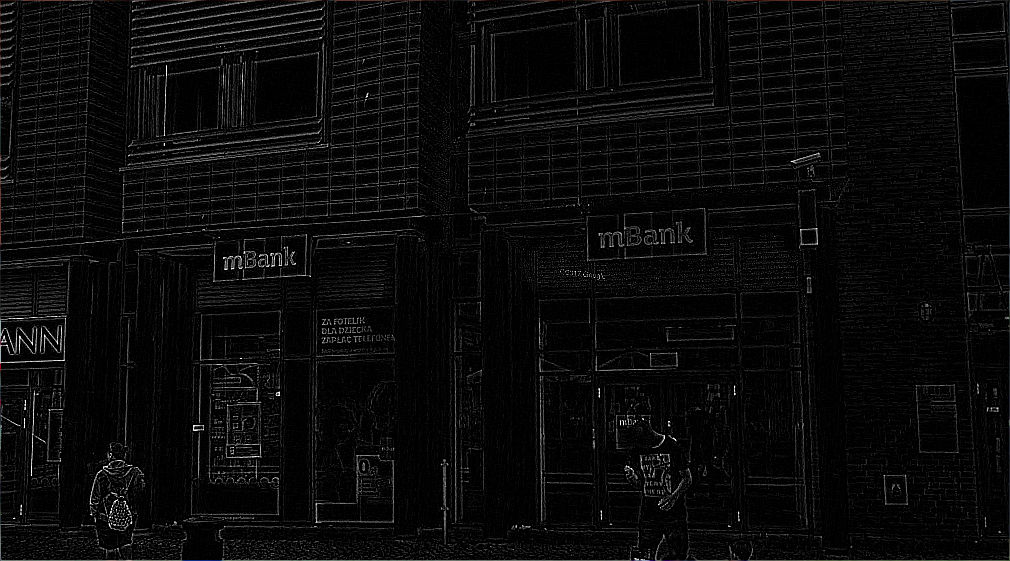
\includegraphics[width=.8\linewidth]{figures/img_sharpened.png}
  \caption{Filtr górnoprzepustowy - zaznaczenie krawędzi}
  \label{fig:sfig2}
\end{subfigure}
\caption{Efekty działania zaimplementowanych filtrów na obrazie d}
\label{fig:filtry}
\end{figure}